\documentclass{article}[18pt]
\usepackage{../../../../format}
\lhead{Networks and Systems - Compiler Design}


\begin{document}
\begin{center}
\underline{\huge Syntax Analysis (Parsing)}
\end{center}
Lexical analyser:
\begin{itemize}
	\item Reads the source program
	\item Produces the sequence of tokens and delivers it to the parser (for syntax analysis)
	\item Tokens are represented by regular expressions
\end{itemize}
Syntax of a programming language:
\begin{itemize}
	\item Expressed by a context free grammar
	\item Alphabet of the grammar - the set of tokens
\end{itemize}
Context free grammar:
\begin{itemize}
	\item A finite way of describing the infinite number of strings
	\item Given by a start symbol and production rules
	\item String - a valid program of the source language
\end{itemize}
Derivation of a string s in grammar:
\begin{enumerate}
	\item Let $A\rightarrow \gamma$ be a production rule
	\item Let $\alpha, \beta$ be strings (with terminals and/or non-terminals)
	\item Then $\alpha A \beta \Rightarrow \alpha \gamma \beta$ means "derives in one step"
	\item $\gamma_1\xRightarrow{*}\gamma_2$ means "derives in zero or more steps"
	\item $\gamma_1\xRightarrow{+}\gamma_2$ means "derives in one or more steps
\end{enumerate}
\section{Derivations}
Grammar:
\begin{center}
	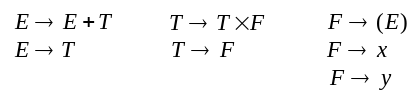
\includegraphics[scale=0.7]{Grammar}
\end{center}
Considering the string $(x+y)\times x$
\begin{center}
	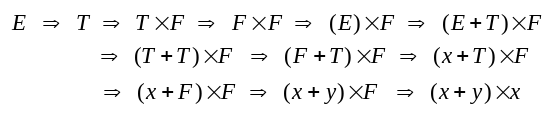
\includegraphics[scale=0.7]{Derivation}
\end{center}
Leftmost derivation - at each stage replace the leftmost non-terminal using a production rule\\
\\
Rightmost derivation - at each stage replace the rightmost non-terminal using a production rule
\section{Parsing}
Purpose of a parser:
\begin{itemize}
	\item Given a string of tokens, to check whether it belongs to the language
	\item If yes, to find a derivation of this string in the grammar
	\item If not, to report useful syntax errors 
\end{itemize}
For well formed strings of tokens (programs):
\begin{itemize}
	\item The parser constructs a syntax tree (parse tree)
	\begin{itemize}
		\item A graphical representation of the derivation of the string in the grammar
	\end{itemize}
	\item The parse tree is passed to the next phase of the compiler (semantic analysis)
\end{itemize}

\begin{center}
	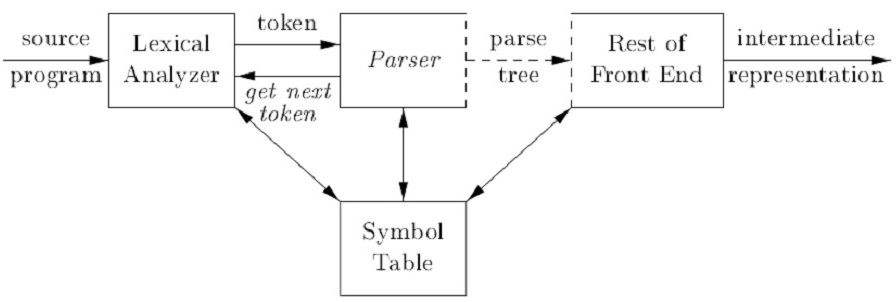
\includegraphics[scale=0.7]{process}
\end{center}
In the parse tree:
\begin{itemize}
	\item Each internal node:
	\begin{itemize}
		\item Is marked by a non-terminal
		\item Represents the application of a production rule
	\end{itemize}
	\item Each leaf is marked by a terminal
	\item All the leaves given the input string
\end{itemize}
Two main methods for constructing a parse tree:
\begin{itemize}
	\item The top-down approach
	\begin{itemize}
		\item Start from the root (labelled with the start symbol)
		\item Continue down to the leaves
	\end{itemize}
	\item The bottom-up approach
	\begin{itemize}
		\item Start from the leaves
		\item Continue up to the root
	\end{itemize}
\end{itemize}
So creating a parse tree from the previous example looks like this
\begin{center}
	\includegraphics[scale=0.7]{"Parse Tree"}
\end{center}
\section{Ambiguity}
Ambiguous grammar:
\begin{itemize}
	\item If there is more than one parse tree for the same string
	\item Equivalently: there exists more than one leftmost (or rightmost) derivation of the same string
\end{itemize}
To prove a grammar is ambiguous just find a string of terminals that is produced by two parse trees\\
\\
A string with two parse trees may have two meanings, therefore we need:
\begin{itemize}
	\item To use additional rules to resolve ambiguities
	\item Or to design unambiguous grammars
\end{itemize}
Common occurrences here are things that are normally solved with BODMAS, e..g what is 9-5+2
\subsection{Resolving ambiguity}
Two solutions:
\begin{itemize}
	\item Use diambiguating rules that "throw away" undesired parse trees
	\item Construct an equivalent unambiguous grammar
\end{itemize}
Example of disambiguating rules:
\begin{itemize}
	\item Impose rules defining the relative precedence of operators when we have two different operators
	\item Operator * has higher precedence than +
\end{itemize}
The dangling else grammar
\begin{center}
	\includegraphics[scale=0.7]{"dangling else"}
\end{center}
Problem - when we read from left to right, which else matches with which else

\begin{center}
	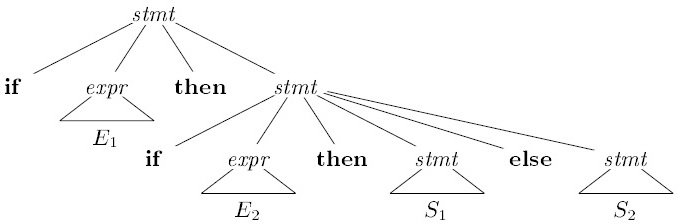
\includegraphics[scale=0.7]{else1}
\end{center}
\begin{center}
	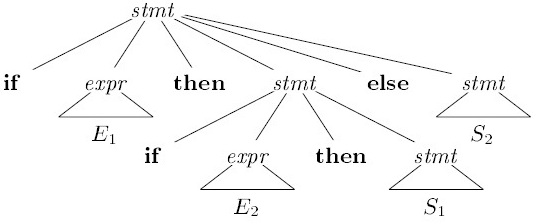
\includegraphics[scale=0.7]{else2}
\end{center}
Most languages prefer the first tree - match each else with the closest unmatched then\\
\\
To rewrite this into an unambiguous grammar
\begin{itemize}
	\item A statement appearing between a then and else must be "matched", i.e. it can't end with an unmatched then
	\item A matched statement is
	\begin{itemize}
		\item Either an if-then-else statement
		\item Or any other unconditional statement
	\end{itemize}
\end{itemize}
\section{Abstract syntax tree}
Recall
\begin{itemize}
	\item The parse tree represents the steps of the derivation of a string
	\item Every internal node:
	\begin{itemize}
		\item Is marked by a non-terminal
		\item Represents the application of a production rule
	\end{itemize}
\end{itemize}
Often parse trees are very complicated
\begin{itemize}
	\item Many non-terminals in the grammar:
	\begin{itemize}
		\item Are auxillary non terminals
		\item Do not represent operations.
	\end{itemize}
	\item We need a simpler representation of string derivations
\end{itemize}
Abstract syntax tree:
\begin{itemize}
	\item Much simpler than the parse tree
	\item Every internal node represents an operation and no a non-terminal
\end{itemize}
\begin{center}
	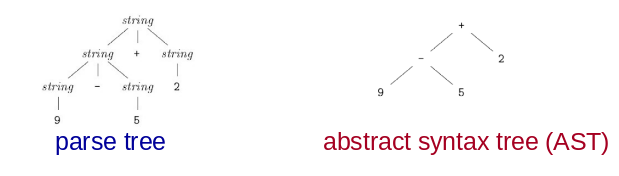
\includegraphics[scale=0.7]{AST}
\end{center}
We can add annotations (or attributes) to the nodes of each tree\\
\\
Attributed:
\begin{itemize}
	\item Detailed information about semantics
	\item e.g. type information, location in memory ...
\end{itemize}



\end{document}